\documentclass[11pt,compress,t,notes=noshow, aspectratio=169, xcolor=table]{beamer}

\usepackage{../../style/lmu-lecture}
% Defines macros and environments
% This file is included in slides and exercises

% Rarely used fontstyle for R packages, used only in 
% - forests/slides-forests-benchmark.tex
% - exercises/single-exercises/methods_l_1.Rnw
% - slides/cart/attic/slides_extra_trees.Rnw
\newcommand{\pkg}[1]{{\fontseries{b}\selectfont #1}}

% Spacing helpers, used often (mostly in exercises for \dlz)
\newcommand{\lz}{\vspace{0.5cm}} % vertical space (used often in slides)
\newcommand{\dlz}{\vspace{1cm}}  % double vertical space (used often in exercises, never in slides)
\newcommand{\oneliner}[1] % Oneliner for important statements, used e.g. in iml, algods
{\begin{block}{}\begin{center}\begin{Large}#1\end{Large}\end{center}\end{block}}

% Don't know if this is used or needed, remove?
% textcolor that works in mathmode
% https://tex.stackexchange.com/a/261480
% Used e.g. in forests/slides-forests-bagging.tex
% [...] \textcolor{blue}{\tfrac{1}{M}\sum^M_{m} [...]
% \makeatletter
% \renewcommand*{\@textcolor}[3]{%
%   \protect\leavevmode
%   \begingroup
%     \color#1{#2}#3%
%   \endgroup
% }
% \makeatother


\title{Interpretable Machine Learning}
% \author{LMU}
%\institute{\href{https://compstat-lmu.github.io/lecture_iml/}{compstat-lmu.github.io/lecture\_iml}}
\date{}

\begin{document}

\newcommand{\titlefigure}{figure_man/shapley_valuefct.png}
\newcommand{\learninggoals}{
\item See prediction as cooperative game
\item Learn about Shapley value to explain individual model predictions
}

\lecturechapter{Shapley Values for Local Explanations}
\lecture{Interpretable Machine Learning}

\begin{vbframe}{Shapley Values}
  We can use Shapley values to explain individual predictions $\fh(\xi)$ of a machine learning model $\fh$:
\begin{itemize}
  \item Players $\hat{=}$ feature values of $i$-th observation $\xi_j, j \in \pset$.
  \item Features cooperate to produce a prediction $\fh(x^{(i)}_1, x^{(i)}_2, \ldots, x^{(i)}_p)$.
  \item The value function / payout of coalition $S$ for observation $\xv^{(i)}$ is
    $$v(S) =  \fh_{S} (\xi_S) - \E (\fh(\xi)),$$ 
    where $\xi_S = \{x_j^{(i)}\}_{j \in S}$ and $\fh_S: \Xspace_S \mapsto \Yspace$.
\item The marginal prediction $\fh_S$ is defined as $\fh_{S}(\xv_S^{(i)}) := \int_{X_C} \fh(\xv_S, X_C)d \P_{X_C}$
\item We have already seen the marginal prediction in action in the PDP.
\item The subtraction of $\E(\fh(\xv))$ is necessary so that $v$ is a value function with $v(\emptyset) = 0$.
\item By using the marginal prediction, we have defined what it means for features to be \enquote{missing} for the prediction: We remove it by integrating over its distribution.
\end{itemize}
\begin{center}
\vspace{-0.3cm}
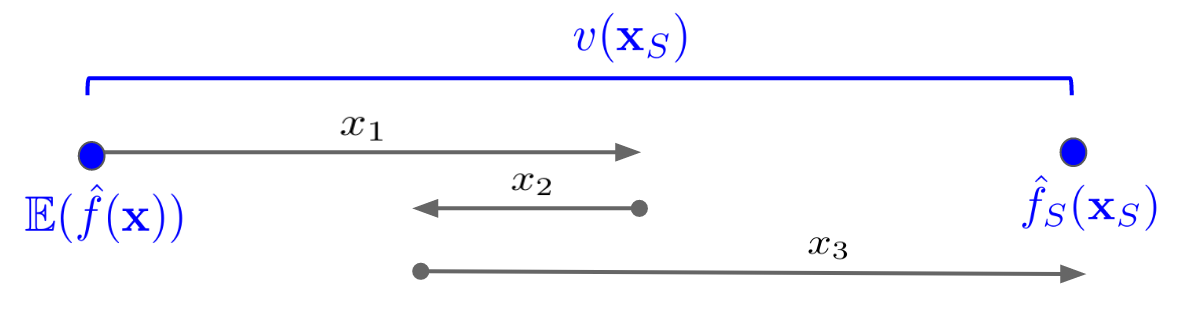
\includegraphics[width=0.6\textwidth]{figure_man/shapley_valuefct}
\end{center}

\begin{itemize}
 \item Shapley values tell us what the payout of each feature is, i.e., how each feature contributes to the overall prediction of a specific observation.
    \item The Shapley value is the average marginal contribution of a feature towards the prediction \textbf{across all possible feature coalitions}.
    \item The sum of Shapley values over all features yields the difference between the average prediction of all data points (baseline) and the selected individual prediction.
  \end{itemize}
\end{vbframe}

\begin{vbframe}{Shapley Value - Definition}
  Using the order definition, the Shapley value for feature $j$ and a given data point $\xi$ can be computed as:

     $$ \phiij  = \frac{1}{p!} \sum_{\Scupj} \underbrace{\fh_{\Scupj}(\xv_{\Scupj}) - \fh_{S}(\xv_{S})}_{\text{marginal contribution of feature $j$}} $$
\begin{itemize}
    \item The term $\E(\fh(\xv))$ drops due to the subtraction of value functions.
  \item Interpretation of Shapley value $\phiij$ for feature $j$ and observation $\xi$:
  The feature value $\xi_j$ contributed $\phiij$ towards the prediction $\fh(\xi)$ compared to the average prediction for the dataset.
   \item Note: Marginal contributions and Shapley values can be negative.
\end{itemize}
\lz
\tiny
Shapley, Lloyd S. 1953. $"$A Value for N-Person Games.$"$\\
\vspace{0.2cm}
Strumbelj, Erik, Igor Kononenko, Erik Strumbelj, and Igor Kononenko. 2014. $"$Explaining prediction models and individual predictions with feature contributions.$"$

\end{vbframe}



\begin{vbframe}{Revisited: Axioms for Fair Attributions}
  We take the general axioms for Shapley Values and apply it to predictions:
  \begin{itemize}
    \item \textbf{Efficiency}: Feature contributions add up to the (centered) prediction. That means, unlike, e.g., LIME, we get a dense attribution, and not a sparse one.
      $\sum\nolimits_{j=1}^p\phi_j=\hat{f}(x)-E_X(\fh(X))$
    \item \textbf{Symmetry}: Two feature that contribute the same to the prediction get the same payout. This ensures that, for example, interaction effects between two features are fairly divided. \\
      $\fh_{S\cup\{j\}}(\xv_{\Scupj}) = \fh_{\Scupk}(\xv_{\Scupk})$ for all $S \subseteq P\setminus\{j,k\}$ then $\phi_j=\phi_k$
    \item \textbf{Dummy / Null Player}: The Shapley value of a feature that does not influence the prediction is zero. This means that if a feature was not selected by the model (e.g., tree or LASSO) the Shapley value is zero.  \\
      $\fh_{\Scupj}(\Scupj)=\fhS(S)$ for all $S \subseteq P$ then $\phi_j=0$
    \item \textbf{Additivity}:  For a prediction with combined payouts, the
      payout is the sum of payouts: $\phi_j(v_1) + \phi_j(v_2)$. This means we can combine the Shapley values for model ensembles.
  \end{itemize}
\end{vbframe}



\begin{vbframe}{Estimation: A practical problem}
  \begin{itemize}
      \item Feature space is often high-dimensional.
      \item High-dimensionality is problematic for the (exact) Shapley value computation: For only 10 features, there are already $10! \approx 3.6$ million possible orders of features.
      \item We have a similar problem with the estimation of the marginal prediction: Averaging over the entire dataset for each (sampled) coalition would be very expensive.
      \item The solution to both problems is sampling. We calculate the Shapley value over $M$ samples. For each sample, we sample one order of features and one data point to replace missing features.
      \item $M$ is a tradeoff between accuracy of the Shapley value and computational costs. The higher $M$, the closer we get to the true Shapley values, but the more costly the computation becomes.
  \end{itemize}
\end{vbframe}

\newcommand{\xk}{\mathbf{x}^{(k)}}

\begin{vbframe}{Estimation Algorithm}
Estimation of $\phi_j$ for model $\fh$, observation $\xi$, and sample size $M$:
  \begin{enumerate}
      \item For m in 1 to M, \textbf{do}:
      \begin{enumerate}
        \item Select random permutation $\pi \in \Pi$.
        \item Select random data point $\xv^{(k)} \in X$.
        \item Order $\xi$ according to $\pi$: $\xi_{\pi} = (x^{(i)}_{\pi(1)}, \ldots, x^{(i)}_{\pi(j)}, \ldots, x^{(i)}_{\pi(p)})$.
        \item Order $\xk$ according to $\pi$: $\xk_{\pi} = (x^{(k)}_{\pi(1)}, \ldots, x^{(k)}_{\pi(j)}, \ldots, x^{(k)}_{\pi(p)})$.
        \item Construct two instances:
          \begin{itemize}
            \item $\mathbf{x}_{+j} = (x^{(i)}_{\pi(1)}, \ldots, x^{(i)}_{\pi(j - 1)}, x^{(i)}_{\pi(j)}, x^{(k)}_{\pi(j + 1)}, \ldots, x^{(k)}_{\pi(p)}) $
            \item $\mathbf{x}_{-j} = (x^{(i)}_{\pi(1)}, \ldots, x^{(i)}_{\pi(j - 1)}, x^{(k)}_{\pi(j)}, x^{(k)}_{\pi(j + 1)}, \ldots, x^{(k)}_{\pi(p)}) $
          \end{itemize}
        \item Compute difference $\phi_j^m = \fh(\mathbf{x}_{+j}) - \fh(\mathbf{x}_{-j})$.
      \end{enumerate}
    \item Compute Shapley value $\phi_j = \frac{1}{M}\sum_{m=1}^M \phi_j^m$.
  \end{enumerate}

  Each $\phi_j^m$ is a sample from the marginal contribution for a sampled coalition.

  \tiny{Strumbelj, Erik, Igor Kononenko, Erik Strumbelj, and Igor Kononenko. 2014. $"$Explaining prediction models and individual predictions with feature contributions.$"$}

\end{vbframe}

\begin{vbframe}{Additional Estimation Trick}


  The Shapley value can be estimated more efficiently when certain coalitions are always included in the computation, instead of relying on chance to sample them.
  \begin{itemize}
    \item The coalition with $S = \emptyset$ (i.e., $|S| = 0$) and $S = \{1, \ldots, p\} \setminus j$ have the highest weights in the Shapley value computation. By including them on purpose, the Shapley value becomes more stable with fewer samples. Sample weights have to be adapted for the sampled coalitions afterwards.
    \item Intuition: Adding a feature to the empty coalition gives information about the \textit{pure} first order effect of the feature, which is the effect without any interactions. Adding the feature value to the otherwise complete set of feature values gives us the information about the total effect of a feature, which is the main effect effect all interaction effects with other features.
    \item For coaliation $S = \emptyset$, there are $0! (|P| - 0 - 1)! = 1 \cdot (|P| - 1)! = (p - 1)!$ orders, which is the same for $S = P \setminus \{j\}$: $|P \setminus \{j\}|! (|P| - |P \setminus \{j\}| - 1)! = (p - 1)! (p - (p-1) - 1)! = (p-1)!$.
    \item An example with $p = 5$ features:
      \begin{itemize}
        \item There are $5! = 120$ orders in total.
        \item In $(5 - 1)! = 24$ orders, we added feature value $\xi_j$ to the empty set.
        \item In 24 orders, we added the feature value to the otherwise full feature set.
        \item That means with just two sets, we can already get $\frac{48}{120} = 0.4$ of the contributions to the Shapley value.
      \end{itemize}
    \item Similarly, we could proceed with all coalitions of $\{S: |S| = 1\}$ and $\{S: |S| = p - 1\}$.
    \item When some coalitions are added \enquote{manually}, and the rest are sampled, we have to adapt the weights: Let $w$ be the weight of the \enquote{manually} sampled coalitions, $\hat{\phi}_{j,fixed}$ the part of the Shapley value with only the manual contributions and $\hat{\phi}_{j,sample}$ the Shapley value with the sampled coalitions, then the Shapley value is: $w \cdot \hat{\phi}_{j,fixed} + (1 - w) \hat{\phi}_{j,sample}$.
  \end{itemize}

  \begin{center}
    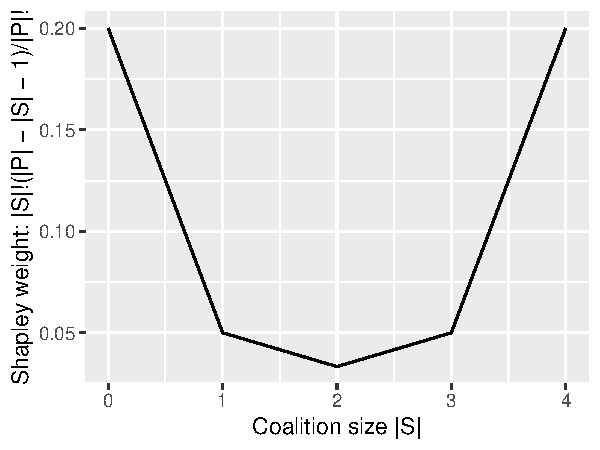
\includegraphics[width=0.5\textwidth]{figure/shapley-weights}
  \end{center}
\end{vbframe}

\begin{vbframe}{Bike Sharing Dataset}

\begin{center}
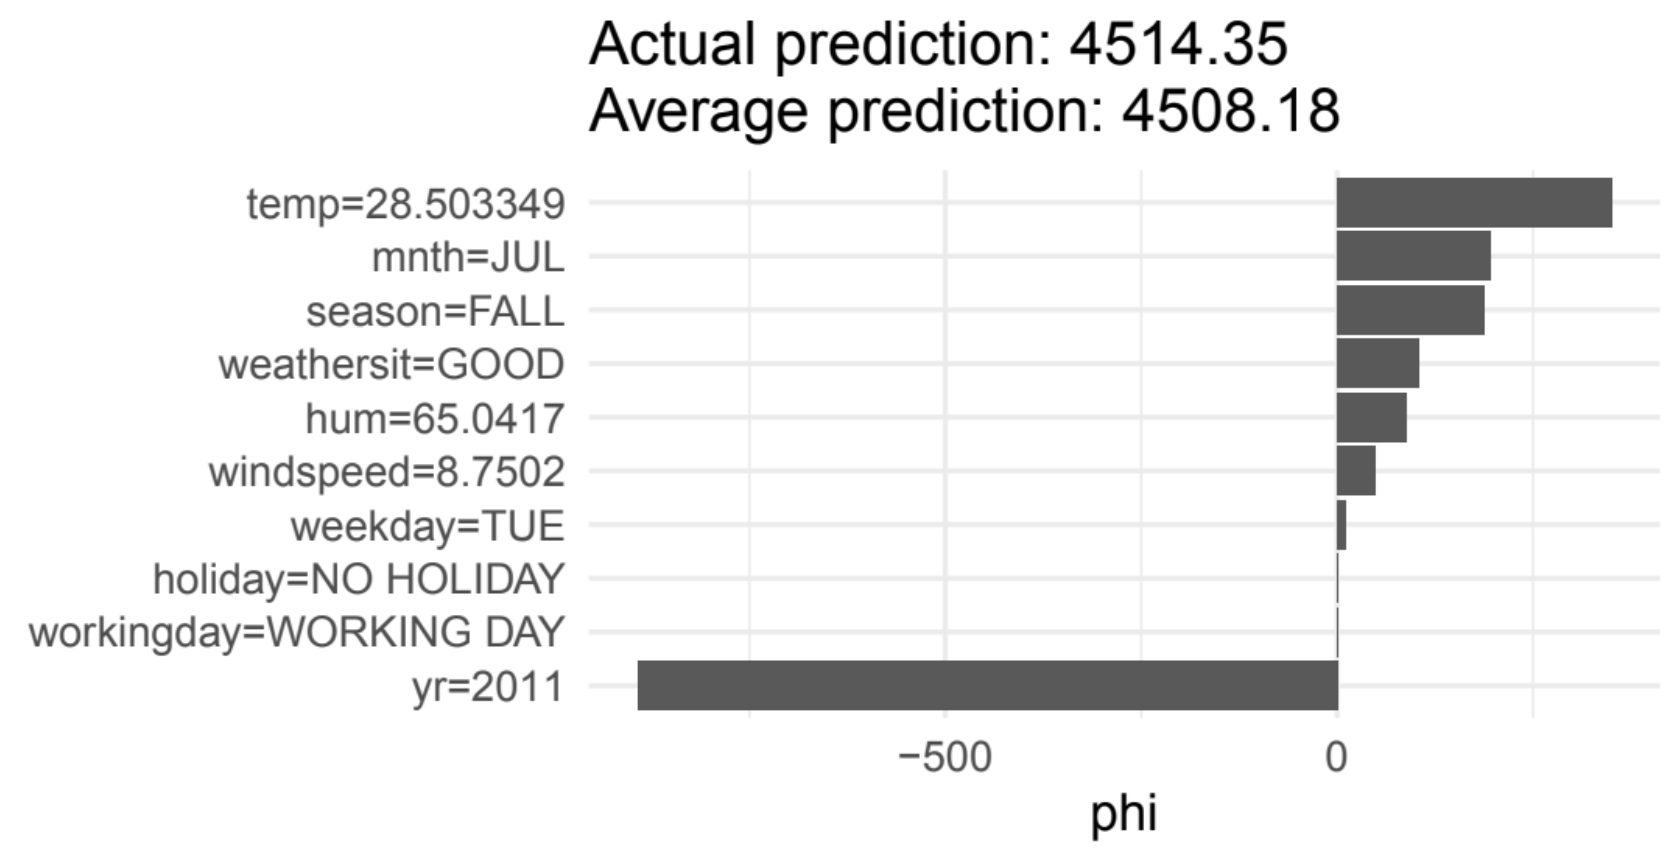
\includegraphics[width=0.85\textwidth]{figure_man/bike-sharing03.png}
\end{center}

The plot shows the Shapley values for observation 200.
The difference between the model prediction of this observation and the average prediction of the data is fairly distributed among the features (i.e., 4514 - 4508).
The most positive effect had feature value temp=28.5, with a contribution (increase of prediction) of + 350.
\end{vbframe}

\begin{vbframe}{Versions of the Shapley Value}

  \begin{itemize}
  \item KernelSHAP formulates the Shapley value solution as a regression problem using a specific kernel function. The authors show paralles to LIME and Deeplift.
  \item TreeSHAP is a fast Shapley value computation method for tree-based models such as gradient boosted trees.
 \end{itemize}
    \tiny{Lundberg, Scott M., and Su-In Lee. "A Unified Approach to Interpreting Model Predictions." Advances in Neural Information Processing Systems 30 (2017): 4765-4774.}
    \tiny{Lundberg, Scott M., Gabriel G. Erion, and Su-In Lee. "Consistent individualized feature attribution for tree ensembles." arXiv preprint arXiv:1802.03888 (2018).}
\end{vbframe}

\begin{vbframe}{ADVANTAGES AND DISADVANTAGES}
	\textbf{Advantages:}
	\begin{itemize}
		\item 	Shapley values are the only explanation method with a solid
		theory. They fulfill various axioms which gives them a reasonable
		foundation.
	\end{itemize}

	\textbf{Disadvantages:}
	\begin{itemize}
		\item 	Without sampling, Shapley values need a lot of computing time to
		inspect all possible coalitions.
		\item The Shapley value of a feature value can be easily misinterpreted:
		It is not the difference of the predicted value after removing the
		feature from the model training; it is the contribution of a feature
		value to the difference between the actual prediction and the mean
		prediction, given the current set of features.
		\item Like many other IML methods, Shapley values suffer from the
		inclusion of unrealistic data instances when features are
		correlated.
	\end{itemize}



\end{vbframe}

\endlecture
\end{document}
